\chapter{Análise e Discussão dos Resultados}

Após o fim dos estudos, iniciou-se a análise das respostas obtidas no questionário aplicado. Todas as perguntas eram opcionais pelo intuito de garantir que apenas respostas de qualidade fossem informadas.

\section{Estudo 1: How do you choose between different Ruby Gems}

Seguem as análises das respostas sobre cada uma das perguntas do questionário `\textit{How do you choose between different Ruby Gems}', com exceção da primeira, sétima e oitava pergunta, pois se tratavam de dados sensíveis dos questionados. 

\subsection{Análise das Respostas}


  \subsubsection{Do you develop software? (Mark all that apply)}

  \begin{itemize}
    \item \textbf{No, I don't}: 0
    \item \textbf{Yes, professionally}: 571
    \item \textbf{Yes, non-professionally}: 402
    \item \textbf{Yes, I contribute to one or more OSS}: 361
  \end{itemize}
  
  \begin{figure}[H]
	\centering
    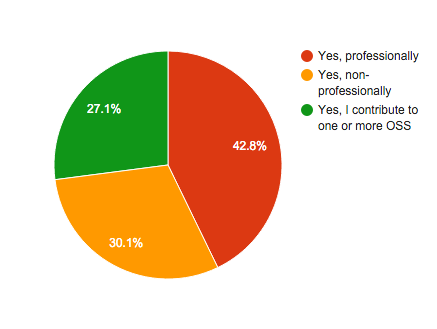
\includegraphics[width=15cm]{Imagens/do-you-develop.png}
    \caption{Do you develop software? (Mark all that apply)}
  \end{figure}
  
  Percebe-se que todos os desenvolvedores tinham algum nível de conhecimento na área de desenvolvimento de software. Além disso, podemos destacar que 85\% deles possuem experiência profissional. Apenas dois usuários não marcaram nenhuma das alternativas.
  
  \subsubsection{How long have you been developing in Ruby?}
  
  \begin{itemize}
    \item \textbf{I don't}: 26
    \item \textbf{Less than a year}: 119
    \item \textbf{1-2 years}: 201
    \item \textbf{2-3 years}: 0
    \item \textbf{3-5 years}: 177
    \item \textbf{More than 5 years}: 141
  \end{itemize}
  
  \begin{figure}[H]
	\centering
    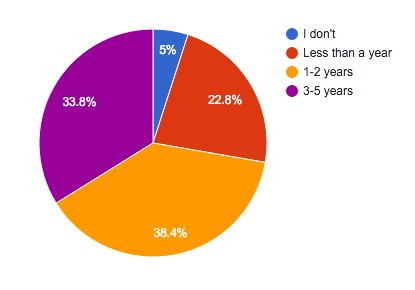
\includegraphics[width=15cm]{Imagens/how-long.png}
    \caption{How long have you been developing in Ruby?}
  \end{figure}
  
  Percebe-se que os desenvolvedores do GitHub, na época do estudo, estavam iniciando com Ruby com no máximo dois anos de desenvolvimento ou já tinham mais experiência com o ambiente com mais de três anos de desenvolvimento. Apenas quatro usuários não marcaram nenhuma das alternativas.

  \subsubsection{When there is more than on gem available that would fulfill your needs - how do you decide which Gem you use?}
  
  Essa pergunta foi a responsável por apresentar os fatores decisivos para a escolha de uma entre duas Gems. Os questionados citaram variadas abordagens onde os fatores decisivos eram indicados por ferramentas ou qualidades.
  
  Para descobrir os principais métodos, ferramentas e qualidades foi utilizado a contagem de palavras nas respostas dos usuários como já citado na metodologia. Dessa forma foi possível convergir os resultados no seguinte \textit{ranking}:
  
  As ferramentas mais citadas, respectivamente foram: GitHub, Ruby Toolbox, Google, RubyGems, Stack Overflow, Rails Casts, Twitter, Blog e IRC.
  
  As qualidades mais citadas, respectivamente foram: Documentação, Atividade, Manutenção, Comunidade, Popularidade, Qualidade, Leia-me, Usabilidade, Testes, Funcionalidade, Cobertura.

\begin{figure}[H]
  \centering
  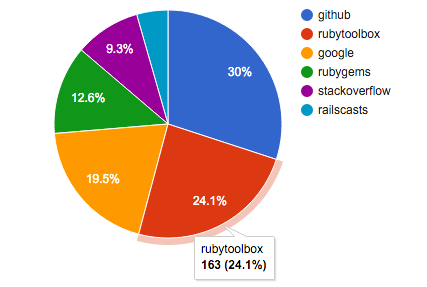
\includegraphics[width=15cm]{Imagens/tools.png}
  \caption{When there is more than on gem available that would fulfill your needs - how do you decide which Gem you use?}
\end{figure}

Assim, percebe-se que desenvolvedores usam bastante ferramentas como o GitHub, Ruby Toolbox e Google. Em particular, a única ferramenta especializada de indicação é o Ruby Toolbox.

\newpage

A seguir as tags utilizadas a fim de localizar as palavras-chave e também as suas menções:

\begin{enumerate}
\begin{multicols}{2}
\item github: 203 menções
\item rubytoolbox: 163 menções
\item google: 132 menções
\item documentation: 120 menções
\item issues: 109 menções
\item rubygems: 85 menções
\item activity: 84 menções
\item stars,forks: 70 menções
\item commit: 66 menções
\item stackoverflow: 63 menções
\item maintained: 59 menções
\item community: 56 menções
\item popular: 48 menções
\item friends: 46 menções
\item quality: 43 menções
\item date: 31 menções
\item dependencies: 31 menções
\item support: 31 menções
\item railscasts: 30 menções
\item blog: 26 menções
\item readme: 24 menções
\item usage: 23 menções
\item tests: 22 menções
\item functionality: 22 menções
\item easy: 21 menções
\item twitter: 20 menções
\item pull requests: 19 menções
\item coverage: 19 menções
\item blog: 19 menções
\item irc: 19 menções
\end{multicols}
\end{enumerate}

\newpage

\subsubsection{What are the most important things you consider when choosing a Gem?}

Usando o processo análogo ao anterior conseguimos o seguinte resultado:

\begin{figure}[H]
  \centering
  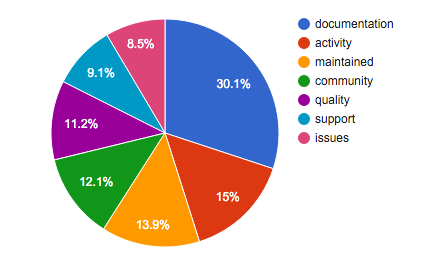
\includegraphics[width=15cm]{Imagens/qualities.png}
  \caption{What are the most important things you consider when choosing a Gem?}
\end{figure}

Percebe-se que documentação, atividade e manutenção é responsável por mais da metade da fatia de qualidades importantes consideradas durante o processo de escolha. Em contra partida, popularidade leva apenas 6\% dos participantes.

\newpage

A seguir as tags utilizadas a fim de localizar as palavras-chave e também as suas menções:

\begin{enumerate}
\begin{multicols}{2}
\item documentation: 166 menções
\item activity: 83 menções
\item maintained: 77 menções
\item community: 67 menções
\item quality: 62 menções
\item github: 55 menções
\item support: 50 menções
\item issues: 47 menções
\item actively: 42 menções
\item popularity: 38 menções
\item recent: 38 menções
\item tests: 35 menções
\item commit: 35 menções
\item coverage: 31 menções
\item forks: 30 menções
\item functionality: 28 menções
\item dependencies: 25 menções
\item stars: 25 menções
\item ease: 24 menções
\item simple: 24 menções
\item examples: 24 menções
\item date: 23 menções
\item features: 23 menções
\item usage: 23 menções
\item popular: 20 menções
\item contributors: 19 menções
\end{multicols}
\end{enumerate}

\newpage

  \subsubsection{Is there room for improvement over the tools you use for finding Gems?}

Quando perguntados se existia espaço para melhoramentos no quesito de busca de Gems, a maioria das respostas se posicionaram de forma negativa, porém com diferentes posturas.

Aqueles questionados que tiveram posturas positivas geralmente também sugeriam funcionalidades adicionais. Algumas dessas funcionalidades encaixavam exatamente com as funcionalidades propostas para a ferramenta.

Foi feito uma tentativa de processar e analisar as mensagens utilizando o Teorema de Bayes a fim de caracterizar se o questionado tinha as suas necessidades atendidas ou não. Além disso também foi feito uma tentativa para elicitar os requisitos dessas mensagens. Ambas tentativas não obtiveram sucesso.

A seguir exemplos de respostas negativas citadas anteriormente: 

\begin{itemize}
	\item \textit{``rubygems.org does a pretty good job with this, at least for my needs.''}
    \item \textit{``I like of the https://www.ruby-toolbox.com/.''}
    \item \textit{``ruby-toolbox.com is pretty good. If there were something that rated documentation and test coverage, those could be useful.''}
    \item \textit{``the great tool called Google combines a lot of these websites together.''}
    \item \textit{``ruby-toolbox.com, it's the best this kind of thing now i think.''}
    \item \textit{``I'm pretty happy with Ruby Toolbox.''}
\end{itemize}

A seguir exemplos de respostas positivas citadas anteriormente: 

\begin{itemize}
	\item \textit{``A tool where developers can give a score to the gems for several points like: code style, code coverage, code architecture, and show the results ordered by any of this ones.''}
    \item \textit{``it would be nice to have reviews on a gem like Amazon does for products.''}
    \item \textit{``I would like something that either categorized them by function or showed most used more accurately''}
    \item \textit{``It's nice to know how active the gem is/how up to date it is.  What issues are people having with it''}
    \item \textit{``There should be webcrawlers rating the Gems around the web using a page-rank algorithm to give insigths on trends, heated discussions, problems on open fórums like StackOverflow, and etc. Like eBay for Gems, where I can use advanced filters to find them.''}
    \item \textit{``I think that ruby gems.org could be improved to a more social network style, with comments, discussions and examples
Searching a Gems for it's name is useless.''}
\end{itemize}

Concluindo a análise do Estudo 1, percebeu-se que a documentação inclusa nos repositórios do GitHub é de extrema importância para qualidade dos projetos. Além disso, percebeu-se que a popularidade é um fator decisivo na escolha de apenas 6\% dos desenvolvedores entrevistados. Como o GitHub não é uma ferramenta especializada na indicação de Gems, ou seja, não possui recomendação baseada em categorias ou funcionalidades, o Estudo 2 foi feito com o seu sucessor o Ruby Toolbox.

\section{Estudo 2: Qual extensão do uso da principal ferramenta}

O Ruby Toolbox usa os índices do GitHub tais como, entre outros, \textit{stars}, \textit{forks} e, de uma forma mais geral, a popularidade dos projetos. Desta forma, foi feito a mineração e então análise dos dados.

O comparativo entre os resultados obtidos está apresentado separado por categorias no Apêndice B. É visível a discrepância das indicações do Ruby Toolbox, com relação ao real uso das Gems, em todas as categorias estudadas exceto nas categorias de \textit{Frameworks} de Teste e Construtores de Formulários. Por exemplo:

\begin{figure}[H]
\centering
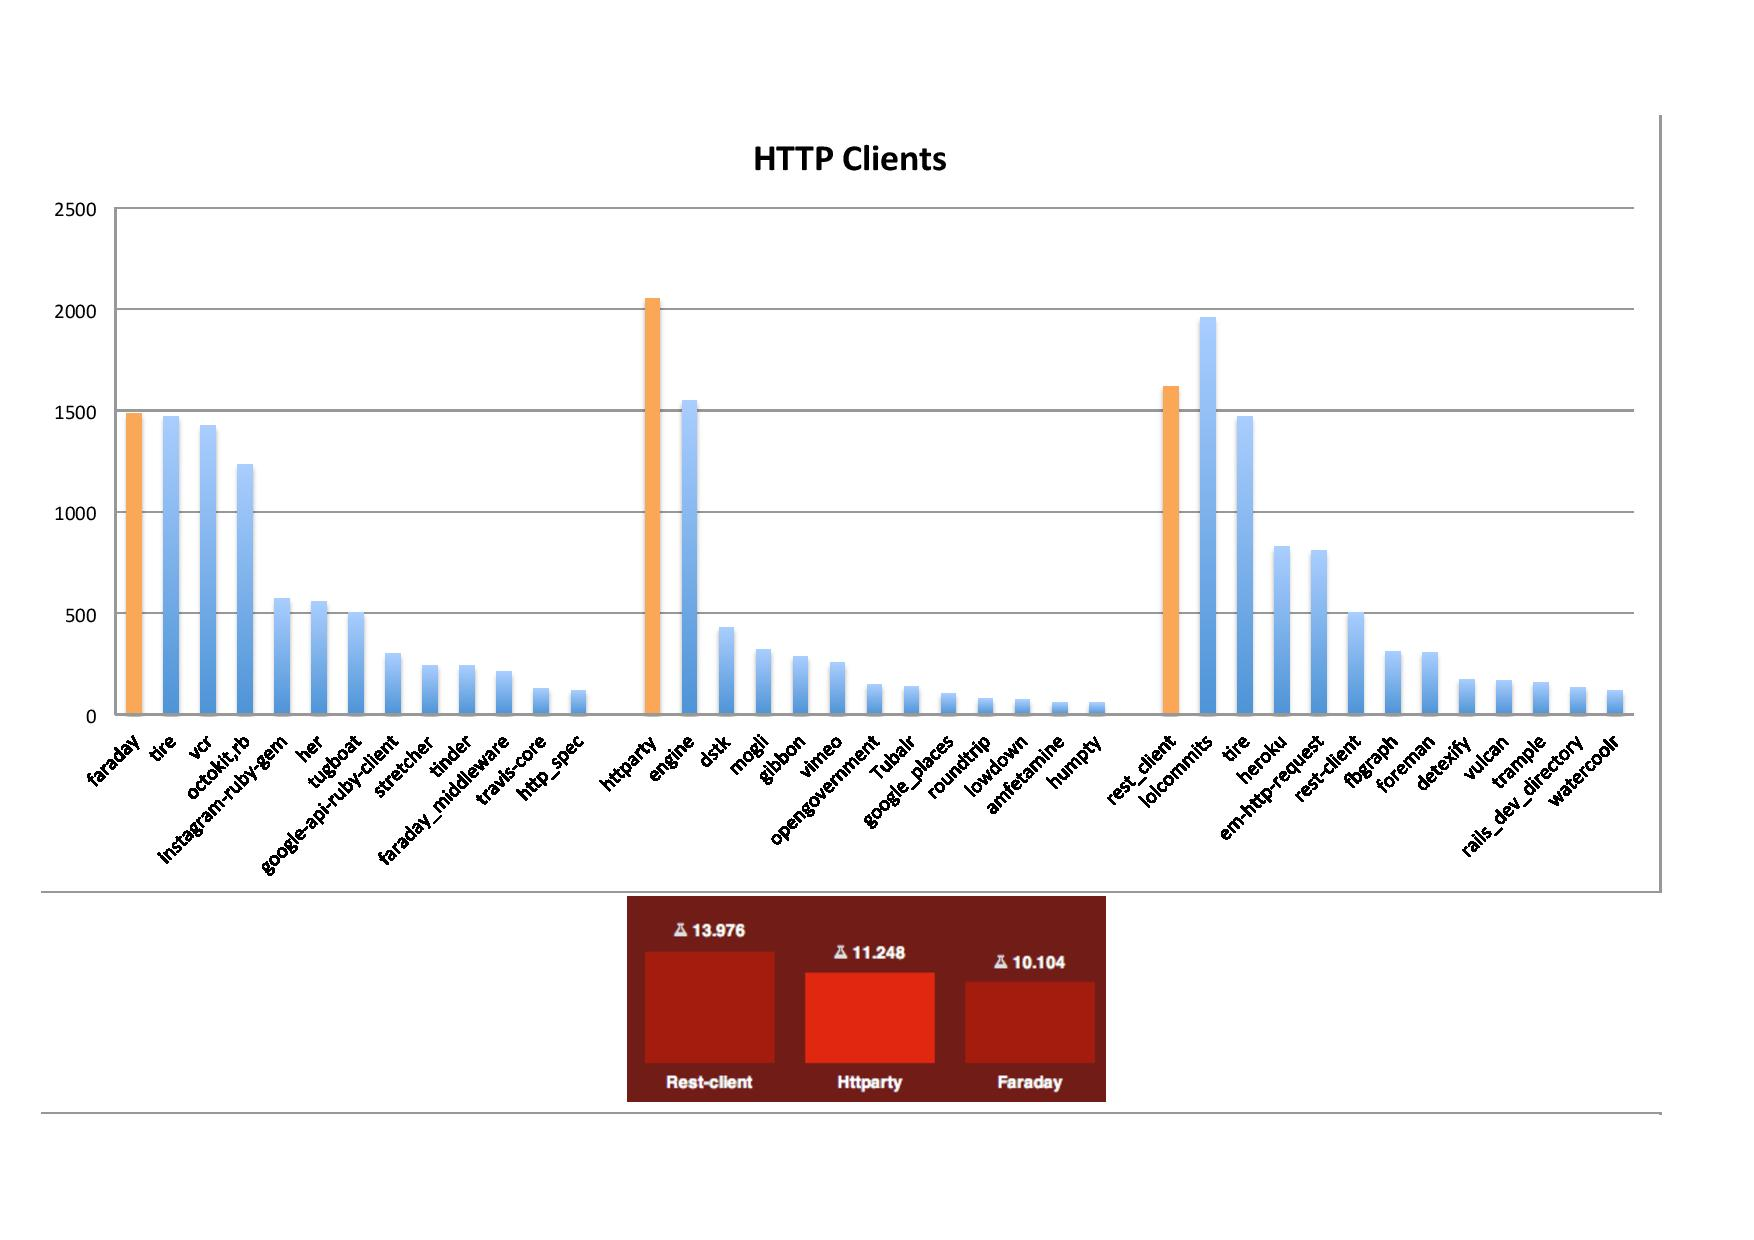
\includegraphics[width=15cm]{Imagens/gems-3.jpg}
\end{figure}

Para a categoria de Clientes HTTP, o Ruby Toolbox indicava respectivamente Rest-client, HTTParty e Farady. Perceba pelo gráfico que HTTParty é amplamente mais utilizado que as outras duas opções. Além disso entre o HTTParty e o Rest-client tem ainda quase duas outras opções.

\section{Estudo 3: Análise da Ferramenta Argue}

Nesta análise cada participante foi anonimado afim de preservar a sua identidade. Toda referência a um participante será feita na forma de P\# onde \# se refere ao identificador do participante.

\subsection{Análise das Respostas}

Segue uma análise detalhada sobre cada uma das respostas feitas.

\subsubsection{Você conhece alguma das gems mencionadas? Comente o que você conhecia sobre cada Gem.}

Com relação ao conhecimento das Gems, 100\% dos participantes que conheciam as Gems já utilizaram Ransack e apenas P2 tinha utilizado ambas Gems.

\begin{itemize}
  \item P1: Sim, ambas. Só ouvi falar sobre ElasticSearch. Já o Ransack está sendo utilizado no projeto em que trabalho.
  \item P2: Sim, ambas. Já trabalhei em pelo menos dois projetos que utilizaram cada uma das gems
  \item P3: Sim, ambas. Utilizei uma delas e ouvi falar de casos de uso da outra
  \item P4: Não
  \item P5: Sim, ambas. Ransack é uma gem para criar formulários de buscas em aplicações Rails. Conheci procurando uma gem que facilitasse a implementação de buscas de modelos através de diversos parâmetros. Acredito que a escolhi por popularidade e facilidade de uso pelo que li da documentação.
  \item P6: Não
  \item P7: Sim, ambas. Já utilizei uma das 2 em 2 projetos.
\end{itemize}

\subsubsection{Algum participante mudou sua opinião a respeito de alguma das gems? Comente sobre a sua escolha}

Após a leitura da discussão ocorreu mudança de opinião apenas nos participantes P1 e P3. Ambos atestaram que a discussão lhe proporcionou mais conhecimentos.

\begin{itemize}
  \item P1: Sim, um. Um dos participantes enfatizou o fato do elasticsearch não ser muito legal para aplicações de pequeno porte.
  \item P2: Não. Ambos falaram coisas certas sobre as duas gems e acredito que cada uma tem um escopo definido, uma não atrapalhando a outra
  \item P3: Sim, um. Sobre a gem que havia utilizado, nada mudou. Porém, o outro participante ofereceu algumas idéias interessantes sobre o uso da outra que ainda não havia pensado ou lido sobre.
  \item P4: Não
  \item P5: Não
  \item P6: Não
  \item P7: Não. Eu ainda acho que cada uma tem seu use case
\end{itemize}

\subsubsection{A partir de agora, você... Comente sobre a sua escolha}

Após o uso da ferramenta 72\% dos questionados afirmaram que, dependendo do contexto, ambas Gems podem ser utilizadas.

\begin{itemize}
  \item P1: Vai usar ambas as gems, de acordo com o contexto
  \item P2: Vai usar ambas as gems, de acordo com o contexto
  \item P3: Vai usar ambas as gems, de acordo com o contexto. Essa já seria minha opção mesmo antes de ler a discussão.
  \item P4: Não vai usar nenhuma das gems
  \item P5: Vai usar somente uma das gems
  \item P6: Vai usar ambas as gems, de acordo com o contexto. Depende muito da aplicação que será desenvolvida e da opinião da equipe de desenvolvimento. Por ter o conhecimento limitado sobre as gems, acredito que é válida a opinião de quem já utilizou e fazer os devidos testes com cada uma.
  \item P7: Vai usar ambas as gems, de acordo com o contexto. Como eu disse, cada uma tem seu use case.
\end{itemize}

\subsubsection{Comente sobre o que você achou da ferramenta.}

\begin{itemize}
  \item P1: \textit{``Achei a ferramente interessante. Seria legal que houvesse um meio de votar em cada um dos argumentos, assim teríamos uma forma de feedback instantâneo sobre a veracidade do argumento, visto que os participantes podem falar o que quiserem (sendo ou não verdade).''}
  \item P2: \textit{``A ferramenta é bem interessante, uma vez que possibilita uma discussão interessante sobre dois tópicos, facilitando a vida de pessoas em busca de qual ferramenta escolher.''}
  \item P3: \textit{``Os participantes poderiam dar uma espécie de "like" para indicar que concorda com o argumento do outro. Poderia haver um campo final para "consenso" onde os dois participantes poderiam escrever um resumo da conversa.''}
  \item P4:
  \item P5: \textit{``Achei prático e interessante.''}
  \item P6: \textit{``É uma ferramenta interessante, a comparação entre ferramentas, frameworks, etc. é um assunto sempre recorrente na área de software. Acredito que um ponto interessante seria destacar melhor os pontos positivos e negativos que cada pessoa possui sobre os objetos de comparação.''}
  \item P7: \textit{``Ficou interessante, dá pra se abordar vários prós e contras de diversas ferramentas.''}
\end{itemize}